\documentclass[acmtocs]{acmtrans2m}

\usepackage[T1]{fontenc}
\usepackage[latin1]{inputenc}
\usepackage{graphicx}
%\usepackage{subfigure}
\usepackage{listings}

\acmVolume{2}
\acmNumber{3}
\acmYear{09}
\acmMonth{09}

\lstset{keywordstyle=\bfseries,
  flexiblecolumns=true,
  showstringspaces=false,
  breaklines=true
}
\lstloadlanguages{[ANSI]C++,HTML}
\lstdefinestyle{prg} {basicstyle=\small\sffamily, showspaces=false}

\newcommand{\prg}[3][tbp]{
\begin{figure}[#1]
  \centering\mbox{\lstinputlisting[language=C++,style=prg]{fig/#2.cc}}
  \caption{#3}
  \label{prg:#2}
\end{figure}
}

\newcommand{\tab}[3][tbp]{
  \begin{acmtable}{8cm}[#1]
    {\centering\small\textsf{\input{fig/#2.tab}}\par}
    \caption{#3}
    \label{tab:#2}
  \end{acmtable}
}

\newcommand{\fig}[4][tbp]{
  \begin{figure}[#1]
    {\centering{\includegraphics[#4]{fig/#2}}\par}
    \caption{#3}
    \label{fig:#2}
  \end{figure}
}


\sloppy

\newcommand{\class}[1]{{\sffamily\bfseries{#1}}}
\newcommand{\method}[1]{\class{#1}}
\newcommand{\us}{$\mu$s}

\markboth{A. Fr�hlich and G. Gracioli}{Periodic Timers Revisited: the
  Real-time Embedded System Perspective}

\title{Periodic Timers Revisited:\\
  the Real-time Embedded System Perspective}

\author{
  ANT�NIO AUGUSTO FR�HLICH and GIOVANI GRACIOLI \\
  Federal University of Santa Catarina
}

\begin{abstract}
  Common sense dictates that single-shot timer mechanisms are more
  suitable for real-time applications than periodic ones, specially in
  what concerns precision and jitter. Nevertheless, \emph{real-time
    embedded systems} are inherently periodic, with tasks whose
  periods are almost always know at design-time. Therefore a carefully
  designed periodic timer should be able to incorporate much of the
  advantages of single-shot timers and yet avoid hardware timers
  reprogramming, an expensive operation for the limited-resource
  platforms of typical embedded systems.

  In this paper, we describe and evaluate two timing mechanisms for
  embedded systems, one periodic and another single-shot, aiming at
  comparing them and identifying their strengths and weaknesses.  Our
  experiments have shown that a properly designed periodic timer can
  usually match, and in some cases even outperform, the single-shot
  counterpart in terms of precision and interference, thus
  reestablishing periodic timers as a dependable alternative for
  real-time embedded systems.

%   In the proposed single-shot timer, a hardware timer is programmed to
%   trigger an interrupt based on the interval to the next event. New
%   events are enqueued according to their relative interval order.  The
%   associated interrupt handler promotes every alarm in the event queue
%   with the time elapsed since the last interrupt, and reprograms the
%   timer with the next event's interval. Conversely, in the proposed
%   periodic timer, the hardware timer is programmed during system
%   initialization to trigger interrupts with a frequency that best
%   matches the periods of events that will be handled by that system.
%   This, in combination with a properly designed event queue, can
%   render a simple, fast, and regular timer interrupt handler.
%   Furthermore, the single-shot timer is limited by hardware
%   resolution, and must fall back to software tick counting when its
%   resolution is exceeded.
\end{abstract}

\category{D.4.7}{Or\-gan\-i\-za\-tion and Design}{Real-time systems
  and embedded systems}


\terms{Design, Performance}

\keywords{Embedded systems, real-time systems, time management}

\begin{document}

\setcounter{page}{111}

\begin{bottomstuff}
  Author's address: Ant�nio Augusto Fr�hlich, Laboratory for
  Software/Hardware Integration, Federal University of Santa Catarina,
  88040-900 Florian�polis, SC, Brazil. %\newline Start of a second footnote ...
\end{bottomstuff}

\maketitle

%------------------------------------------------------------------------- 
\section{Introduction} \label{sec:intro}

% - What is timing about?
The notion of time is essential to any real-time embedded system. The
system needs to keep track of time flow to schedule tasks and also to
provide time services, such as delays and alarms, to applications.

% - How timing has been done in ordinary OS?
Historically, operating systems have been implementing time management
almost in the same way: a hardware timer is configured to periodically
trigger interrupts, thus giving rise to a system time unit called
\emph{tick}. Ticks define the minimum perception of time flow within
the system and rule every sort of time-driven events. The mechanism is
usually implemented with a single hardware timer, whose interrupt
handler is overloaded with operations around task scheduling and timed
event propagation.

% - Criticize periodic timer and introduce single-shot
Though well-accepted in the realm of general-purpose systems, time
management strategies based on periodic timers face strong criticism
from the real-time system community~\cite{Regehr:2005}. For instance,
in a system with a periodic timer configured to generate 10ms ticks, a
15ms delay request may result, in the worst case, in a waiting time of
30ms\footnote{If the request is posted just after a tick is generated,
  counting will start on the next tick. Moreover, 15 might be rounded
  up to 20, yielding a total wait of 30ms.}. In addition to the lack
of precision in time services, the periodic timer handler is
constantly activated, even if no action needs to be taken, causing
overhead and interference for the running tasks.  These limitations
fostered the mechanism of \emph{single-shot} timer, with dedicated
timers being programmed to fire exactly when an action has to be
performed~\cite{Aron:2000,Tsafrir:2005,Goel:2002}.

% - Rescue periodic timer
Nonetheless, despite these unquestionable issues about periodic
timers, while performing experiments in the context of a previous
paper~\cite{SCCC:2008}, we realized that single-shot supremacy might
be indeed more closely connected to implementation issues than to the
concept itself. Some of the aspects that called our attention were:

\begin{itemize}
\item Real-time embedded systems are intrinsically periodic. Even
  simple software architectures, such as cyclic executives, have a
  period derived from the main loop length. Real-time scheduling in
  more complex embedded systems is essentially periodic (e.g.,
  Earliest Deadline First, Rate Monotonic, etc).

\item Single-shot timers are usually multiplexed on a few physical
  timers, demanding constant hardware reprogramming, what, in some
  systems is much slower than software reprogramming.

\item Single-shot timers, in practice, do overflow, demanding some sort
  of periodic fall-back mechanism.
\end{itemize}

In this way, a carefully designed periodic timer mechanism could, in
theory, incorporate much of the advantages of single-shot timers.
Indeed, even commercial operating systems now feature improved
periodic timers: Windows Vista can adjust the period of the hardware
timer according to the system load~\cite{Peter:2008}; Linux delivers a
secondary high resolution timing interfaces to
applications~\cite{Siddha:2007}. Therefore, this paper investigated
this hypothesis by comparing the behavior of both time management
strategies (i.e., periodic and single-shot) in the same scenario
(i.e., hardware platform, operating system, and applications). Our
results confirmed that a properly configured and implemented periodic
timer may yield high precision and low overhead. Single-shot timers,
on the other hand, are usually able to match the precision of periodic
timers, and can cause less interference in the system when a periodic
timer is not well-configured.

The remainder of this paper is organized as follows:
section~\ref{sec:rel} presents related work; section~\ref{sec:design}
presents the design and implementation of single-shot and periodic
timing mechanisms; section~\ref{sec:case} describes the experimental
evaluation of proposed mechanisms, along with a comparative analysis;
section~\ref{sec:con} closes the paper with our final considerations.

%------------------------------------------------------------------------- 
\section{Related Work}\label{sec:rel}

Tsarfrir et. Al. discuss some issues of periodic time management, as
lack of precision, and power consumption~\cite{Tsafrir:2005}. This
work proposes a solution based on \emph{Smart Timers}, which have
three basic properties: 1) Accurate timing with configurable maximum
latency; 2) Reduced management overhead by triggering combined nearby
events, and (3) Reduced overhead by avoiding unnecessary periodic
events.

Kohout presents a strategy to efficiently support real-time OS, using
core components implemented in hardware~\cite{Kohout:2003}. The main
objective is to reduce the impact caused by the real-time OS in the
application. This impact is measured in terms of response time and CPU
usage. This work introduces the Real-Time Task Manager (RTM), 
a memory-mapped on-chip task manager designed to deal with task scheduling,
time management and event management. The RTM support for time management
functions causes a 10\% reduction of CPU time (with 24 tasks).

Aron and Druschel introduced the concept of \emph{Soft-Timer}, which
triggers the time manager in the return of every system call, and not
only in the hardware timer events.  These results have shown a
reduction in the number of context switches, and an increase in the
time service precision, since system calls tend to be much more
frequent than timer interrupts. Although system calls are widely
executed in every system, its rate is not predictable. Therefore this
approach cannot guarantee continuous precision, and periodic timer
interrupts are used to satisfy minimum operating system requirements.

Goel et Al. combined three different time management approaches
(single-shot timer, soft-timer, and periodic timer) to build an
efficient, high-resolution, low-overhead mechanism they called
\emph{Firm Timer}. The combination allows for a reduction in the
number of timer interrupts, thus reducing the overall overhead of
periodic timers in the system~\cite{Goel:2002}.

In summary, all these works focus on eliminating the side-effects
associated to the maintenance of a global system's tick counter.  In
particular, activation of the timer interrupt handler solely to
increment the tick counter is strongly avoided. For this purpose,
single-shot mechanisms are proposed. The performance evaluation of
such mechanisms, however, is mostly done in the context of
general-purpose systems, disregarding hardware reconfiguration times
and the periodic nature of real-time embedded systems.

%------------------------------------------------------------------------- 
\section{Design and Implementation} \label{sec:design}

The design and implementation of the single-shot timer and periodic
timer were carried out in the Embedded Parallel Operating System
(\textsc{Epos})~\cite{Froehlich:2001,Marcondes:ETFA:2006}. EPOS is a
multi-platform, component-based, embedded system framework, in which
traditional operating system services are implemented through
adaptable, platform-independent \emph{System Abstractions}.
Platform-specific support is implemented through \emph{Hardware
  Mediators}~\cite{PolpetaF04}.  Mediators are functionally equivalent
to device drivers in \textsc{Unix}, but do not build a traditional
\emph{Hardware Abstraction Layer}~(HAL). Instead, they sustain the
interface contract between abstractions and hardware components by
means of static metaprogramming techniques, thus ``dissolving''
mediator code into abstractions at compile-time.

Time is managed in \textsc{Epos} by the families of components shown
in Figure~\ref{fig:epos_time}. The \class{Clock} abstraction is
responsible for keeping track of the current time, and is only
available on systems that feature a real-time clock device, which is
in turn abstracted by a member of the \class{RTC} family of mediators.
The \class{Chronometer} abstraction is used to measure time intervals,
through the use of a timestamp counter (\class{TSC}) mediator. If a
given platform does not feature a hardware timestamp counter, its
functionality may be emulated by an ordinary periodic timer.

\fig{epos_time}{\textsc{Epos} timing components.}{scale=.75}

The \class{Alarm} abstraction can be used to generate timed events,
and also to put a thread to \emph{sleep} for a certain time.  For this
purpose, an application instantiates a handler and registers it with
an Alarm specifying a time period and the number of times the handler
object is to be invoked. \textsc{Epos} allows application processes to
handle events at user-level through the \class{Handler} family of
abstractions depicted in Figure~\ref{fig:epos_handler}. The
\class{Handler\_Function} member assigns an ordinary function supplied
by the application to handle an event. The \class{Handler\_Thread}
member assigns a thread to handle an interrupt. Such a thread must
have been previously created by the application in the suspended
state. It is then resumed at every occurrence of the corresponding
event. Finally, the \class{Handler\_Semaphore} assigns a semaphore,
previously created by the application and initialized with zero, to an
event. The operating system invokes operation \method{v} on this
semaphore at every event occurrence, while the handling thread invokes
operation \method{p} to wait for an event.

\fig[b]{epos_handler}{\textsc{Epos} event handlers.}{scale=.75}

Although not in the scope of this work, it is worth to mention that
the same mechanisms are used in \textsc{Epos} for real-time thread
scheduling.

Figure~\ref{fig:class_diagram} presents the class diagram of
\class{Alarm} and \class{Chronometer} abstractions for the AVR-8
architecture. The \class{Alarm} abstraction uses two of the hardware
timers available in the AVR microcontroller. One of these timers,
\class{ATMega128\_Timer\_3}, is used to control the \class{Alarm}
request queue. With the system clock configured at 7.2 MHz and a
prescale of 1024, this 16-bit timer allows the scheduling of events
spanning approximately 9 seconds.  The other timer,
\class{ATMega128\_Timer\_1}, generates periodic interrupts that
trigger the system scheduler. These interrupts only occur when the
scheduler is active, with a period that corresponds to the system's
configured \emph{quantum}.

\fig{class_diagram}{Class diagram of \textsc{Epos} abstractions and
  mediators for the AVR-8 architecture.}{width=\columnwidth}%{scale=.75}

Figure~\ref{prg:time_app} illustrates how an application uses time
services in the \textsc{Epos} system. This application reads current
system time through a \class{Clock} object, measures time intervals
with a \class{Chronometer}, and registers a periodic \class{Alarm}
with an associated \class{Handler\_Function}.

\prg{time_app}{Example of time service utilization in \textsc{Epos}.}

The \class{Timer} class abstracts timing hardware.  In a periodic
event model, the platform's timer is set with a constant
(configurable) frequency. When a new alarm event is registered, its
interval is converted to timer \emph{ticks}, with $ T = \frac{I}{F} $,
where $T$ is the number of ticks, $I$ is the desired interval, and $F$
is the timer frequency. The event is then inserted into an ordered and
relative request queue. Thus, manipulation of this queue affects only
its head, because it keeps all values relative to the first element.
Due to rounding errors, the number of ticks may not correspond to the
exact desired interval. When a timer interrupt is triggered, an
interrupt handler, registered by the \class{Alarm} abstraction,
increments the tick counter, thus promoting every alarm in the event
queue by a tick. If the event at the head of the queue has no more
ticks to count, its handler is released. The corresponding interrupt
handler is depicted in the UML sequence diagram of
Figure~\ref{fig:handler_periodic}.

% \begin{lstlisting}[language=C++,style=prg]
%   //decrease one tick from the queue head element
%   if(requests_queue.head()->promote() <= 0) {
%       // process the alarm queue
%       // trigger current event 
%   }
% \end{lstlisting}

\fig{handler_periodic}{Periodic alarm handler sequence
  diagram.}{scale=.5}

In this work, we designed and implemented a new event model, based on
\emph{single-shot} timers. In a single-shot model, the platform's
timer is programmed based on the interval to the next event. New
events are enqueued according to their relative interval order.  The
\class{Alarm} interrupt handler promotes every alarm in the event
queue with the time elapsed since the last interrupt, and reprograms
the timer with the next event's interval. Since in this scheme there
are no conversions between intervals and ticks, precision loss is
restricted to physical timer resolution.

In order to generate interrupts at a given frequency, hardware timers
are usually configured with a frequency prescaler (relative to
processor clock), and a comparison register. The hardware timer counts
a tick at each clock period, and triggers an interrupt when the ticks
counter reaches the value in the comparison register.  Valid hardware
periods are given by the following equation:

\begin{equation}
\frac{D}{C}  \leq  P \leq  \frac{D \times (2^{r} - 1)}{C} 
\label{eq:period}
\end{equation}

\noindent where $D$ is the clock prescaler, $C$ is the system's clock
frequency, $P$ is the timer's period, and $r$ is the timer's
resolution. Thus, when the desired event interval is larger than the
timer's hardware resolution, the \class{Timer} mediator needs to count
ticks in software.

In order to allow waiting for a period larger than the hardware timer
resolution, without incurring in overhead when this is not necessary,
we introduced a \method{MAX\_PERIOD} \emph{configuration trait} to the
timer implementation. This trait allows compile-time specialization
for either hardware or software based counting, as necessary. When
software counting is activated, the \class{Timer} mediator handles its
own interrupt, in which it increments a tick counter. When this
counter is equal to the desired period, a new interrupt is triggered
by the software, to be handled by the \class{Alarm} abstraction. As
was the case with periodic timers, there may be rounding errors
introduced by the conversion from period to ticks. Since the interrupt
to be handled by the \class{Alarm} changes according to configuration,
the timer informs its IRQ through a class method.  The corresponding
interrupt handler is depicted in the UML sequence diagram of
Figure~\ref{fig:handler_single-shot}.

% \begin{lstlisting}[language=C++,style=prg]
%   Queue::Element * e = requests_queue.head();
%   Microsecond elapsed_time = e->rank(); 
%   e->promote(elapsed_time); 
%   if(e->has_times_to_execute)
%         //reinsert the alarm in the queue
%   if(!requests_queue.empty()) 
%         // calculate the time to next event
%         timer.period(_requests.head()->rank());
%   // trigger current event 
% \end{lstlisting}

\fig{handler_single-shot}{Single-shot alarm handler sequence
  diagram.}{scale=.5}

%------------------------------------------------------------------------- 
\section{Experimental Evaluation}\label{sec:case}

In order to evaluate the proposed time management strategies, we
devised some experiments. Our first experiment was targeted at
measuring the actual period of events with distinct periods, in
different timer clock configurations.  Figure~\ref{prg:alarm} presents
the application implemented for this test. The main thread creates an
alarm event with several iterations, and waits for the completion of
all handlers. For each test, the period of each event was configured
with a different value, from 100~$\mu$s to 10~s. Each event handler
stores the timestamp of its execution instant. The difference between
two consecutive timestamps results in an interval that, ideally,
should be equal to the requested event period.

\prg{alarm}{Periodic alarm application.}

\tab{error_periodic}{Difference between expected and measured periods
  using periodic timer.}

\tab{error_single-shot}{Difference between expected and measured
  periods using single-shot timer.}

For every period and clock frequency, the periodic timer's frequency,
and the single-shot timer's maximum period were configured with
\emph{ideal} values. Thus, for example, if the event's period was 1~s,
the periodic timer's frequency was set to 1~Hz, and single-shot
timer's maximum period was set to 1~s. From this follows that,
whenever possible, the periodic timer's behavior was equivalent to
that of a single-shot timer: the timer's interrupt is only triggered
when there is an event to run. Likewise, the single-shot timer's
implementation only falls back to software tick counting when strictly
necessary (i.e. when the requested event period is larger than the
hardware's resolution). Thus, our tests yield the best possible
results for each timing strategy.

We executed this experiment in an 8-bit AVR microcontroller, with a
16-bit timer/counter.  We configured this timer with three different
clock frequencies: 7200~Hz, 28800~Hz, and 115200~Hz.
Tables~\ref{tab:error_periodic} and \ref{tab:error_single-shot}
present the average total period of each event, configured with
different clock frequencies, in each timing strategy. It should be
noted that, while the single-shot timing strategy usually presents
better results than its periodic equivalents, both strategies present
considerable errors for short periods when a ``slow'' (e.g. 7200~Hz)
timer clock is used.  Furthermore, when the requested period exceeds
the maximum hardware period, and the single-shot timer falls back to
software tick counting, errors for this strategy increase
considerably. Likewise, when using a very ``fast'' (e.g. 115200~Hz)
timer clock, the overhead of reprogramming the single-shot timer may
exceed the overhead of counting ticks in periodic timers. Finally, it
should be noted that these values represent a best-case scenario for
periodic timers, since the timer's period was configured as close to
the event's period as possible. Nonetheless, these values represent a
typical case for single-shot timers whenever the maximum event period
is smaller or equal to the maximum timer hardware period.

\fig{error}{Error rates for different periods.}{width=\columnwidth}

Figure~\ref{fig:error} presents error curves (actual period relative
to ideal period) for each tested period, in each clock configuration,
for each timing strategy. In every case, the error rates decrease as
the requested period increases, and as the timer's clock speed
increases.  With larger periods and faster timer clocks, the overhead
and rounding errors of the timing system are minimized. The upwards
slope in the single-shot tests represents the moment where the timer's
hardware maximum period is exceeded, and the timer falls back on
software tick counting.

While a periodic timer may have equivalent or even superior
performance than a single-shot timer, its implementation may interfere
with other parts of the system. A single-shot timer only generates
interrupts when there is an event to be handled, while a periodic
timer generates interrupts at a constant rate, regardless of whether
there is an event to handle or not.  Thus, a periodic timer service
may interfere with other threads in the system. In order to evaluate
this phenomenon, we measured the time spent in handling an alarm event
in both approaches using the same AVR platform. At the beginning of
the alarm handler, we turned a led on and before leaving the handler
we turned it off. We plugged the output of the led to a digital
oscilloscope to measure the elapsed time.  For this test, an alarm
triggered at every 5ms and the timer was configured with a frequency
of 1000~Hz and a clock of 125000~Hz. A periodic timer generates four
interrupts before the alarm is released, that is, during 4 interrupts
it will only count ticks.  The single-shot timer only triggers when it
is necessary, but it must reprogram the timer after each event. The
goal of the experiment is to measure the interference of both
approaches in the system as a whole. Obtained values are shown in
Table~\ref{tab:handler_time}.  For an interrupt that counts ticks, the
periodic timer took 14~\us{} and for an interrupt where is necessary
to release the alarm it took 42~\us{}.  The single-shot timer,
however, took 212~\us{} for releasing the alarm event. This high
overhead is due the time needed to reprogram the hardware timer.

\tab{handler_time}{Time spent in handling the alarm interrupt using
  periodic and single-shot timers.}

In order to evaluate the behavior of a poorly configured periodic
timer, we devised a simple actuation system, in the form of a
\emph{Pulse-Width Modulator} ~(PWM) software application. In this
application, a thread ``glows'' the leds at different intensities
along the time (Figure~\ref{prg:leds}).  An alarm event periodically
changes the intensity of each led (duty cycle).  In order to create
the illusion of glowing, the main thread must be executed at a regular
period, with no interruptions other than the one that changes the
intensity of each led.

\prg{leds}{PWM led glowing application.}

We executed this application on the same AVR platform. The event period
for the alarm that changes leds intensity was set to 20~ms. The timer's
clock was set to 125000~Hz, and the periodic timer's frequency was set
to 1000~Hz (1 interrupt at every 1~ms), 500~Hz (1 interrupt at every
2~ms) and 50~Hz (1 interrupt at every 20~ms, the best case for the
periodic timer). Figure~\ref{fig:interference} shows the interference
caused by the timer mechanisms on period of the thread that handles the
leds. In order to measure this period, the output of one of the leds was
connected to a digital oscilloscope. Note that the small period variance
for single-shot is not related to interrupt handling interference, but
to the very own nature of the PWM algorithm.

Figure~\ref{fig:deviation} summarizes the interference caused by timers
mechanisms on the period of the PWM thread in terms of standard
deviation. When the single-shot timer was used, the thread's average
period was 40.52~\us{}, with a standard deviation of 1.12~\us{} (2.77\%
of the thread's average period). When the 1000~Hz periodic timer was
used, the average period of this thread was 40.75~\us{} with a standard
deviation of 1.72~\us{} (4.23\% of the thread's average period). Since
the periodic timer is not well configured, it generates interrupts that
interfere with application.  On the other hand, the periodic timers
configured with 500~Hz and 50~Hz presented average periods of
40.51~\us{} and 40.44~\us{} respectively, but the 500~Hz periodic timer
obtained a higher standard deviation (1.19~\us{} of the thread's average
period).  Since the 50~Hz periodic timer will only generate interrupts
when necessary, it presented the best average period and standard
deviation.  This example shows how a bad periodic timer configuration
can affect the system performance.

\begin{figure}
\centering
\begin{tabular}{cc}
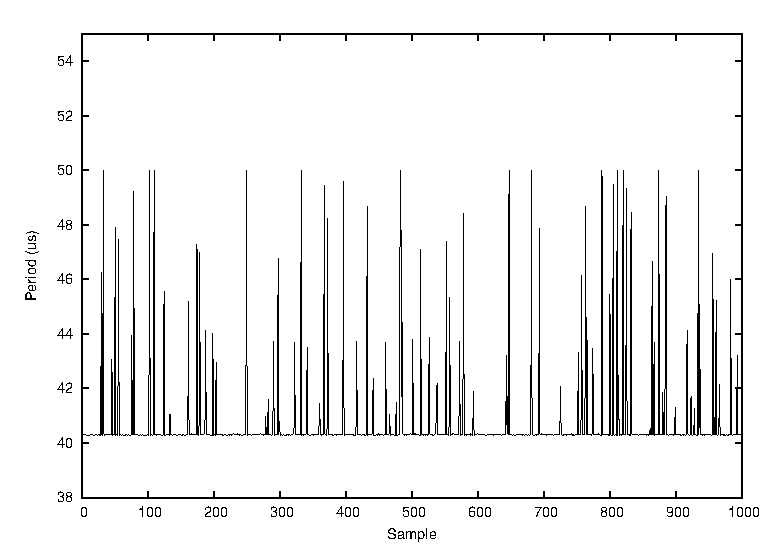
\includegraphics[scale=0.47]{fig/interference_periodic_1000hz} &
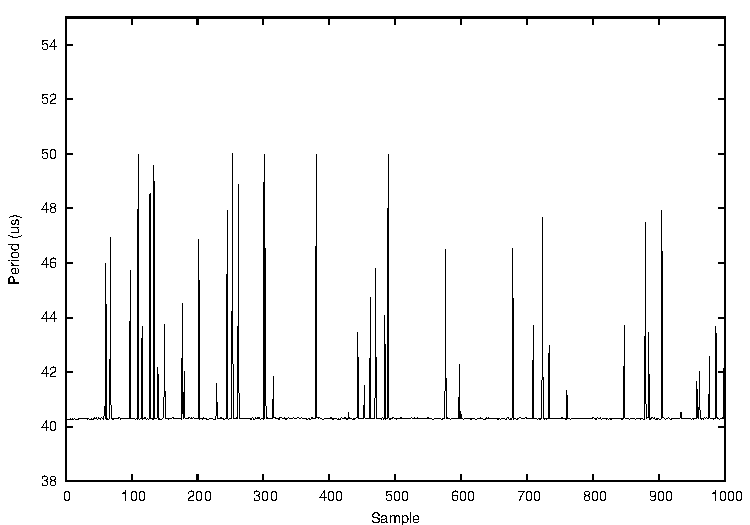
\includegraphics[scale=0.47]{fig/interference_periodic_500hz}\\
(a) Periodic timer at 1000Hz & (b) Periodic timer at 500Hz\\
\\
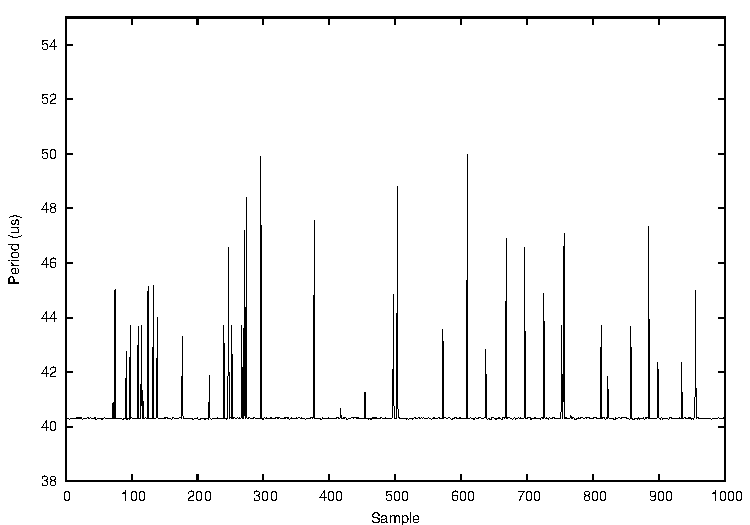
\includegraphics[scale=0.47]{fig/interference_periodic_50hz} &
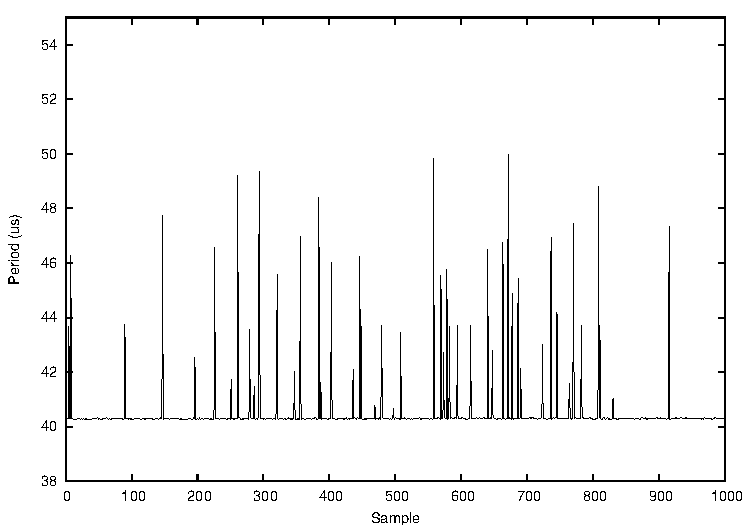
\includegraphics[scale=0.47]{fig/interference_single-shot} \\
(c) Periodic timer at 50Hz & (d) Single-shot \\
\end{tabular}
\caption{Timer interference on the PWM thread's period along the time: (a)
  using periodic timer configured with 1000Hz; (b) periodic timer with
  500Hz; (c) periodic timer with 50Hz; and (d) using single-shot
  timer.}
\label{fig:interference}
\end{figure}

\fig{deviation}{Mean period and standard deviation for each timer
  strategy and configuration with relation to
  Figure~\ref{fig:interference}.}{scale=0.75}

Two final remarks about the experiments carried out:

\begin{itemize}
\item Deeply embedded system

  Our work focused on deeply embedded systems. Such systems present
  serious resources limitations, such as power consumption, processing
  power and memory. Moreover, these systems are designed to run a
  specific set of applications, whose requirements are known at
  design-time. Therefore, configuring the periodic timer to fit system
  needs is a fully valid approach.

  Furthermore, the time spent by reprogramming the hardware timer in
  the single-shot implementation in deeply embedded system is high,
  since this task involves calculations, like divisions and
  multiplications, in order to adjust the next time requested by the
  application to the hardware timer period.

\item \textsc{Epos} dependency

  The experiments described here used the \textsc{Epos} system, but
  the basic idea can be applied to virtually any embedded operating
  systems. The problem itself is related to how the periodic timer is
  implemented and not to the embedded operating system. A smart
  periodic time management implementation can supply and adjust to the
  needs of embedded or real-time applications.
\end{itemize}


%------------------------------------------------------------------------ 
\section{Conclusion}\label{sec:con}

Common sense dictates that single-shot timer mechanisms are better
than periodic ones. Nonetheless, our experiments have shown that, for
real-time embedded systems, a properly configured periodic timer can
usually match the single-shot approach in terms of performance and
interference.  Indeed, they shown that a periodic timer can, in some
specific cases, outperform an equivalent single-shot mechanism. This
apparently unaccountable outcome arises basically from the
intrinsically periodic nature of embedded systems and from the way
timers are implemented in such systems.

A periodic timer mechanism does not require the hardware timer to be
reprogrammed for each event. In a periodic timer, the hardware timer
is programmed during system initialization to trigger interrupts with
a frequency that best matches the periods of events that will be
handled by that system. This, in combination with a properly designed
event queue, can render a simple, fast, and regular timer interrupt
handler.  Furthermore, a single-shot timer is limited by hardware
resolution, and must fall back to software tick counting when its
resolution is exceeded.

Although this scenario of tailored periodic timer mechanisms does not
fit the all-purpose essence of ordinary operating systems, which must
work in a best-effort to accommodate a myriad of application demands,
it does fit quite well in the realm of real-time embedded systems. It
is not our intention, however, to promote periodic timers as a
generally better alternative for such systems than single-shot.  There
are many cases in the literature for which single-shot approaches have
proved superior, in particular, concerning power efficiency and
jitter. Our main intention is to reestablish periodic timer mechanisms
as a concrete alternative for real-time embedded systems.

%------------------------------------------------------------------------ 
\begin{acks}\label{sec:ack}

  We would like to thank and acknowledge LISHA members Lucas Wanner,
  Roberto de Matos and Danillo Moura Santos for the work on the
  initial implementation of single-shot timers for \textsc{Epos} and
  for the assistance with the experiments reported in this paper. We
  would also like to thank Prof.~R�mulo de Oliveria for the prolific
  discussions about timing in real-time systems.

\end{acks}

\bibliographystyle{acmtrans}
\bibliography{timing}

\begin{received}
Received June 2009;
November 1993;
accepted January 1996
\end{received}

\end{document}
